\section{KHO DỮ LIỆU}

\subsection{Khái niệm}
Kho dữ liệu (Data Warehouse - DW) là tập hợp dữ liệu có đặc tính: Hướng chủ đề, Tích hợp, Ổn định và Biến thiên theo thời gian, nhằm mục đích hỗ trợ phân tích và ra quyết định quản trị.

\subsection{Phân biệt CSDL Tác nghiệp (OLTP) và Kho dữ liệu (OLAP)}
\begin{table}[H]
    \centering
    \renewcommand{\arraystretch}{1.3}
    \begin{tabularx}{\textwidth}{|p{2.8cm}|X|X|}
        \hline
        \textbf{Đặc điểm} & \textbf{CSDL Tác nghiệp (OLTP)} & \textbf{Kho dữ liệu (OLAP)} \\
        \hline
        \textbf{Mục đích} & Xử lý giao dịch hàng ngày & Phân tích, báo cáo, hỗ trợ ra quyết định chiến lược. \\
        \hline
        \textbf{Dữ liệu} & Dữ liệu hiện tại, chi tiết, cập nhật liên tục. & Dữ liệu lịch sử, tổng hợp, ít thay đổi. \\
        \hline
        \textbf{Thời gian} & Tốc độ xử lý giao dịch rất nhanh. & Truy vấn phân tích phức tạp, tốn nhiều thời gian hơn. \\   
        \hline
        \textbf{Cấu trúc} & Chuẩn hóa cao để tránh dư thừa. & Phi chuẩn hóa để tối ưu đọc. \\
        \hline
        \textbf{Thao tác} & Chủ yếu là Insert, Update, Delete. & Chủ yếu là Select, Aggregation. \\
        \hline
    \end{tabularx}
\end{table}

\subsection{Đặc tính cốt lõi của Kho dữ liệu}
\begin{enumerate}
    \item Hướng chủ đề: Dữ liệu được tổ chức theo các chủ đề chính (Khách hàng, Sản phẩm, Doanh thu...).
    \item Tích hợp: Dữ liệu được làm sạch và thống nhất từ nhiều nguồn khác nhau.
    \item Biến thiên theo thời gian: Luôn gắn liền với yếu tố thời gian.
    \item Ổn định/Bất biến: Dữ liệu sau khi đưa vào kho thường không bị sửa đổi hay ghi đè, chỉ đọc.
\end{enumerate}

\subsection{OLAP (Online Analytical Processing)}
\begin{itemize}
    \item Khái niệm: Công nghệ cho phép người dùng phân tích dữ liệu đa chiều một cách tương tác và nhanh chóng.
    \item Phân biệt: OLTP dùng để ghi dữ liệu (Insert/Update), OLAP dùng để đọc và phân tích đa chiều (Select/Aggregation).
    \item Ví dụ: Xem doanh thu theo Vùng miền và Thời gian.
\end{itemize}

\subsection{Kiến trúc Kho dữ liệu}
Kiến trúc bao gồm các thành phần chính: Nguồn dữ liệu; Trích xuất, Chuyển đổi và Tải dữ liệu; Kho dữ liệu trung tâm; Các kho dữ liệu nhỏ; Các công cụ phân tích dữ liệu.

\begin{figure}[H]
    \centering
    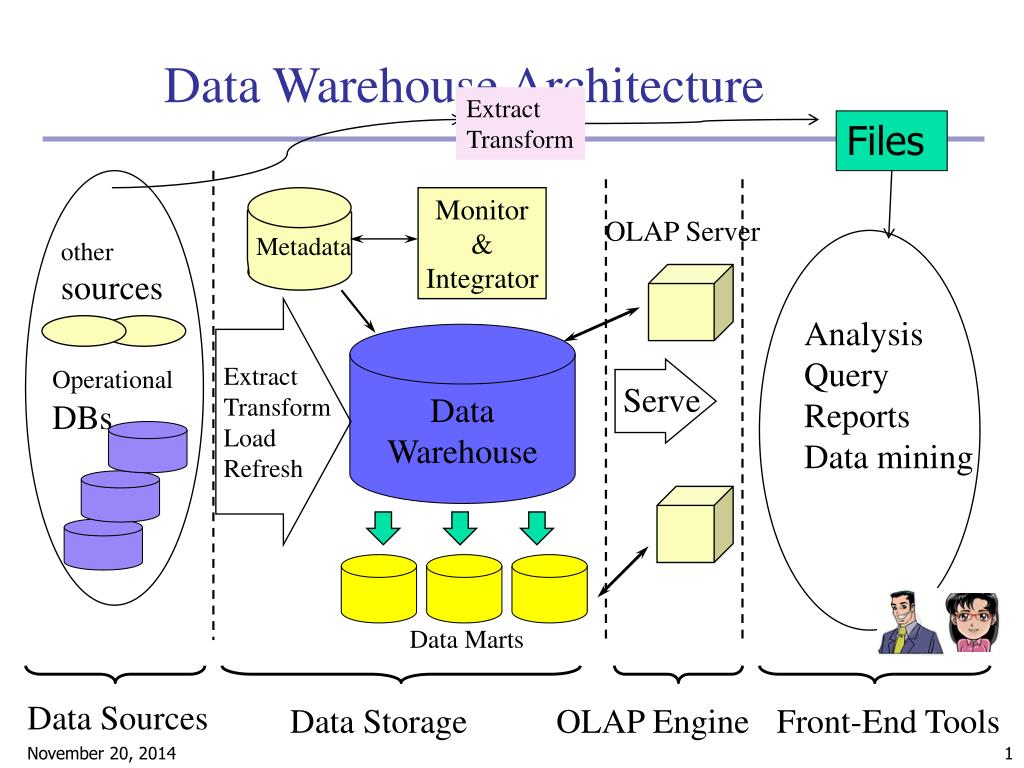
\includegraphics[width=1\textwidth]{figures/DW/Data_Warehouse.jpg}
    \caption{Kiến trúc Data Warehouse}
    \label{fig:data-warehouse}
\end{figure}

\subsection{Quy trình xây dựng}
Quy trình: (1) Xác định yêu cầu; (2) Thiết kế mô hình đa chiều; (3) ETL; (4) Triển khai; (5) Kiểm thử - bảo trì.

\subsection{Mô hình hóa Kho dữ liệu}
\begin{itemize}
    \item Mô hình Ngôi sao : Cấu trúc đơn giản nhất. Một bảng sự kiện Fact ở trung tâm, kết nối trực tiếp với các bảng chiều Dimension xung quanh. \textit{Ưu điểm:} Truy vấn cực nhanh, dễ hiểu.
    \item Mô hình Thiên hà : Đây là kiểu mô hình chứa vài bảng Fact và chia sẻ các bảng Dimension. \textit{Ưu điểm:} Giảm kích thước của cơ sở dữ liệu, tiết kiệm bộ nhớ.
    \item Mô hình Bông tuyết : Là dạng mở rộng của lược đồ hình sao bằng cách bổ sung các Dimension. Bảng Fact giống lược đồ hình sao. Bảng Dim được chuẩn hóa. Các chiều được cấu trúc rõ ràng. \textit{Ưu điểm:} Tiết kiệm bộ nhớ.
    \item Mô hình Chòm sao : Phức tạp nhất. Gồm nhiều bảng Fact chia sẻ chung bảng Dimension. \textit{Ứng dụng:} Hệ thống lớn.
\end{itemize}

\begin{figure}[H]
    \centering
    \begin{tabular}{cc}
        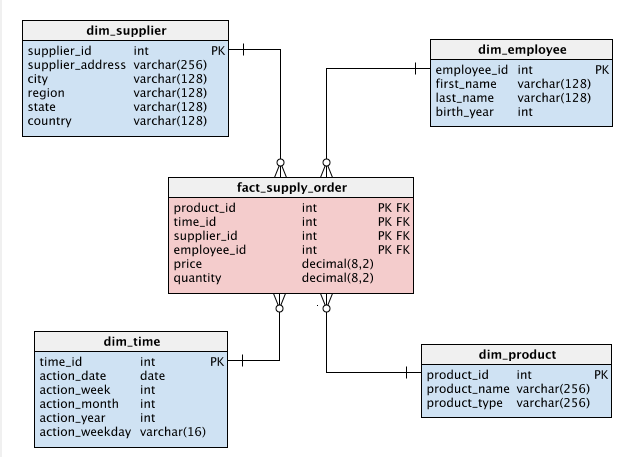
\includegraphics[width=0.45\textwidth,height=0.27\textheight,keepaspectratio]{figures/DW/Supply_Orders.png}
        &
        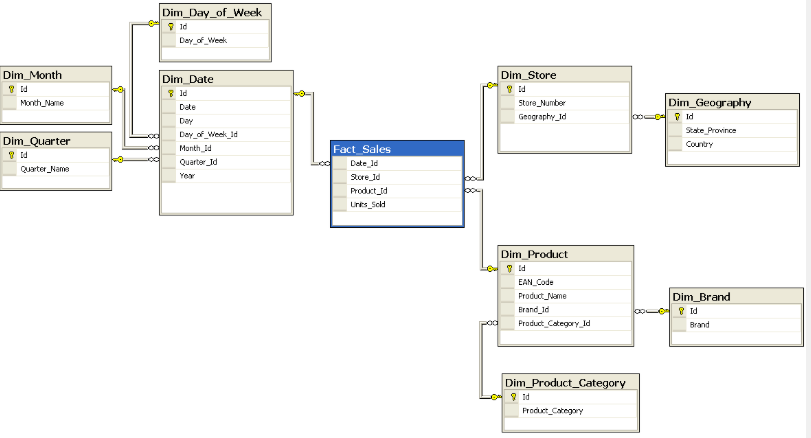
\includegraphics[width=0.45\textwidth,height=0.27\textheight,keepaspectratio]{figures/DW/Snowflake_Schema.png}
        \\
        \textbf{Mô hình Ngôi sao}
        &
        \textbf{Mô hình Bông tuyết}
        \\[0.8em]
        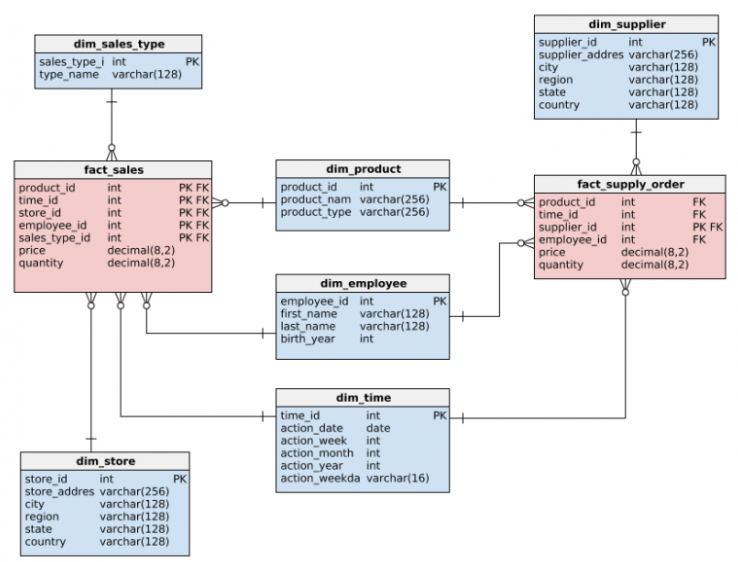
\includegraphics[width=0.45\textwidth,height=0.27\textheight,keepaspectratio]{figures/DW/Galaxy_Schema.png}
        &
        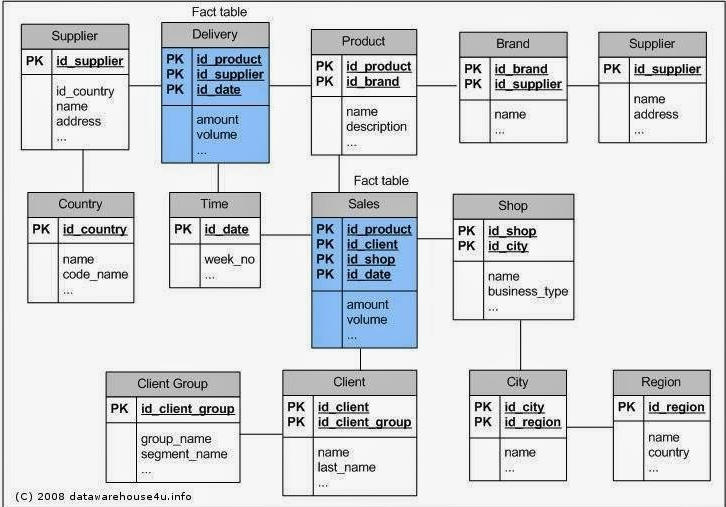
\includegraphics[width=0.45\textwidth,height=0.27\textheight,keepaspectratio]{figures/DW/Constellation_Schema.png}
        \\
        \textbf{Mô hình Thiên hà}
        &
        \textbf{Mô hình Chòm sao}
    \end{tabular}
\end{figure}
